\begin{figure}[!ht]
\centering
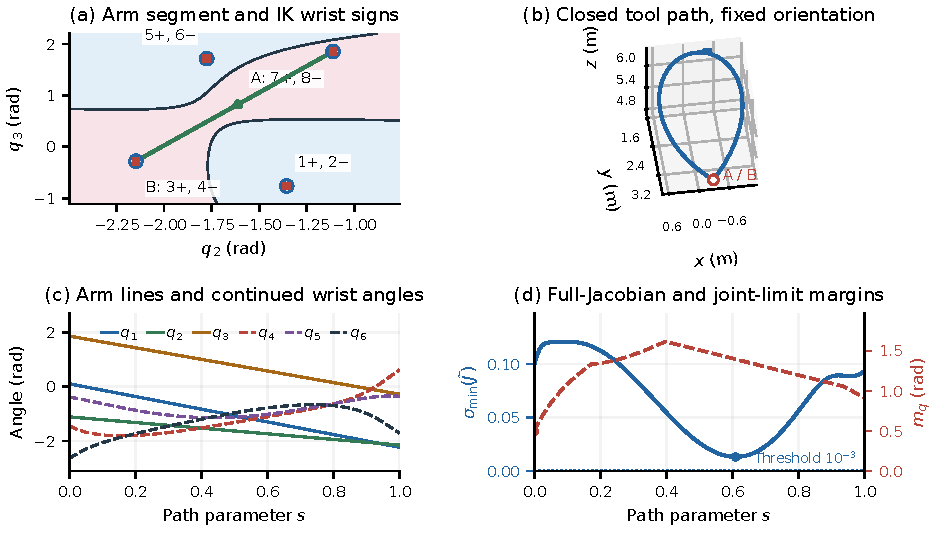
\includegraphics[width=\linewidth]{figures/connectivity_linear.pdf}
\caption{Arm singularities and a fixed-orientation solution change
in (a) joint space and (b) the wrist-centre workspace,
with $\rho_w=\sqrt{x_w^2+y_w^2}$.
The cusps indicate that the CuRo6R's positioning chain is cuspidal: it can
change between IK solutions without crossing an arm singularity.
At the marked target, $t_1<t_2<t_3<t_4$.
The folds $F_{ij}$ merge $t_i,t_j$; cusps $C_k$ are indexed by the
root $k$ shared by their incident folds, with $u/r$ superscript distinguishing upper/right.}
\label{fig:arm-singularity-map}
\label{fig:connectivity-linear}
\end{figure}

\textbf{A straight arm path with fixed tool orientation.} We index each full configuration $\vect{q}^{(i)}$ by its arm root $t_i$
on the chosen wrist branch. We choose the initial joint configuration
$\vect{q}^{(4)}=(0.1024,\allowbreak-1.1124,\allowbreak1.8547,\allowbreak-1.4399,\allowbreak-0.3835,\allowbreak-2.6486)^\trans$
(in radians), compute ${}^0T_{E,d}=\operatorname{FK}(\vect{q}^{(4)})$, and solve the IK
for this pose, obtaining eight solutions. Excluding the initial solution,
exactly one has the same signs of $\det J_{v,\mathrm{arm}}$ and $\sin q_5$:
$\vect{q}^{(2)}\approx(-2.2287,\allowbreak-2.1482,\allowbreak-0.2788,\allowbreak0.6181,\allowbreak-0.3524,\allowbreak-1.7072)^\trans$.
This candidate also satisfies the endpoint joint-limit and singularity
margins, but matching signs alone does not guarantee a nonsingular connection.

We discretize the straight path between their arm joints
$\vect{q}_a=(q_1,q_2,q_3)^\trans$:
\begin{equation}
 \vect{q}_a(s)=(1-s)\vect{q}_a^{(4)}+s\vect{q}_a^{(2)},\qquad 0\leq s\leq1,
 \label{eq:connectivity-arm-segment}
\end{equation}
where $s$ measures path advancement. At each sample, we remove the arm
orientation from the desired orientation ${}^0R_{E,d}$ by computing
${}^3R_{E,d}(s)=({}^0R_3(\vect{q}_a(s)))^\trans\,{}^0R_{E,d}$.
We recover the wrist angles using \eqref{eq:ik-wrist-solutions}, preserving
the initial sign of $\sin q_5$ and choosing continuous angle representatives.
The tool orientation remains fixed while its position is free to vary.

We continue only while joint-limit clearance is nonnegative, the arm
determinant retains its sign, $|\sin q_5|>10^{-6}$, and
$\sigma_{\min}(\widetilde J)>10^{-3}$, where
$\widetilde J=\operatorname{diag}(\ell_c^{-1}I_3,I_3)\,{}^0J_E$
uses the characteristic length $\ell_c=2\,\mathrm m$ to scale the linear
velocity rows. A failed check stops the attempt; acceptance also requires
reaching the selected goal. Figure~\ref{fig:connectivity-linear} shows the
accepted change from $\vect{q}^{(4)}$ to $\vect{q}^{(2)}$. These checks concern the sampled
configurations, so a finer discretization improves confidence of real success.
